\documentclass[11pt, a4paper]{report}
\usepackage[utf8]{inputenc}
\usepackage{graphicx}
\usepackage{amsmath}
\usepackage{geometry}
\geometry{margin=1in}

\begin{document}

\begin{titlepage}
    \centering
    
\includegraphics[width=0.7\textwidth]{amrita_logo.png} % Replace with the correct logo file if needed
    \vspace{0.5cm}
    
    {\Large \textbf{AMRITA VISHWA VIDYAPEETHAM}}\\
    \vspace{0.2cm}
    {\large Deemed to be University under Section 3 of UGC Act, 1956}
    \vspace{1.5cm}
    
    {\Huge \textbf{Project 1: Recommender System }}\\
    \vspace{2cm}
    
    {\large \textbf{Submitted By:}}\\
    \vspace{0.5cm}
    {\Large \textbf{Ajithkumar A K}}\\
    \textbf{[CB.AI.R4CEN24009]}\\
    \vspace{2cm}
    
    {\large \textbf{Supervisor:}}\\
    \vspace{0.5cm}
    {\Large Dr. Soman K P}\\
    \vspace{2cm}
    
    {\large Submitted to}\\
    {\large \textbf{Amrita Vishwa Vidyapeetham, University}}\\
    {\large Amrita School of Artificial Intelligence}\\
    \vspace{2cm}
    
    {\large Submission Date: \textbf{November 21, 2024}}
\end{titlepage}

\begin{document}

\maketitle

\pagenumbering{roman}
\tableofcontents
\chapter{Recommendation Systems: Implementation and Analysis}

\section{Summary}
This project focuses on implementing and analyzing recommendation systems, a vital component in personalization and user experience across various domains like e-commerce, streaming platforms, and content curation. The primary purpose is to predict user preferences based on available data and suggest items they are likely to engage with, using three key approaches:

\section{Collaborative Filtering}
\begin{itemize}
    \item This method calculates user-user similarity to predict missing ratings for items based on the preferences of similar users.
    \item A global baseline approach is also implemented, which accounts for overall average ratings and user-item biases to improve prediction accuracy.
\end{itemize}

\section{Singular Value Decomposition (SVD)}
\begin{itemize}
    \item SVD is used to reduce the dimensionality of the user-item matrix, capturing latent factors that influence user preferences while retaining 90\% of the original data's energy.
    \item This approach is computationally efficient and effective for sparse datasets.
\end{itemize}

\section{CUR Decomposition}
\begin{itemize}
    \item CUR involves sampling rows (users) and columns (items) to approximate the user-item matrix.
    \item Two sampling techniques are explored:
    \begin{itemize}
        \item Sampling with replacement.
        \item Sampling without replacement.
    \end{itemize}
\end{itemize}

\section{Dataset Description}
The project uses the Jester Online Joke Recommender Dataset, a robust dataset with 4.1 million continuous ratings (-10.00 to +10.00) from 73,421 users for 100 jokes. Data preprocessing, including handling missing ratings and normalization, ensures the dataset is ready for analysis.

\section{Outcomes}
\begin{itemize}
    \item \textbf{Collaborative Filtering:} Showed robust performance in predicting missing ratings, especially with dense regions of the dataset.
    \item \textbf{SVD:} Achieved efficient dimensionality reduction, balancing computational cost with prediction accuracy.
    \item \textbf{CUR:} Provided flexible matrix approximations, offering insights into row and column sampling strategies.
\end{itemize}

\section{Evaluation Metrics and Insights}
The evaluation metrics, including Normalized Mean Absolute Error (NMAE), precision, recall, and F1 score, demonstrate the strengths and trade-offs of each approach. The project highlights the adaptability of these methods in addressing challenges like sparse data and computational constraints, offering a solid foundation for enhancing recommender systems.

\chapter*{Abstract}
This project aims to develop and evaluate a recommender system using collaborative filtering, Singular Value Decomposition (SVD), and CUR decomposition techniques. The objective is to predict missing user ratings and suggest items based on user preferences. The dataset used is the Jester Online Joke Recommender Dataset, containing 4.1 million ratings from 73,421 users for 100 jokes, with ratings ranging from -10.00 to +10.00. 

The project implements:
\begin{itemize}
    \item Collaborative filtering based on user similarity and a global baseline approach.
    \item SVD for dimensionality reduction.
    \item CUR for matrix approximation through row and column sampling.
\end{itemize}

The key findings highlight:
\begin{itemize}
    \item Collaborative filtering and SVD are effective for sparse datasets.
    \item CUR provides a flexible, computationally efficient alternative.
\end{itemize}

Evaluation metrics such as Normalized Mean Absolute Error (NMAE), precision, and recall demonstrate the strengths and trade-offs of each algorithm, providing insights into their applicability in real-world recommendation systems.

\chapter{Introduction}

Recommender systems are algorithms designed to predict and suggest items (products, movies, songs, etc.) to users based on their preferences, past behavior, or similarities with other users. They have become a crucial part of the modern digital landscape, providing personalized experiences in e-commerce, streaming platforms, and content curation services. By helping users discover relevant content from large datasets, recommender systems enhance user engagement, satisfaction, and conversion rates. For example, in e-commerce, they suggest products that users are likely to purchase, while on streaming platforms like Netflix or Spotify, they recommend movies or music based on individual tastes.

\section{Types of Recommender Systems}

\begin{itemize}
    \item \textbf{Collaborative Filtering (CF):} \\
    Collaborative filtering is based on the idea that users who have agreed in the past will agree in the future. It operates by comparing a user's preferences with those of other users and recommending items that similar users have liked. There are two main types of collaborative filtering:
    \begin{itemize}
        \item \textit{User-based CF:} Identifies users who are similar to the target user and recommends items based on what those similar users have liked.
        \item \textit{Item-based CF:} Finds items similar to the ones the user has already rated highly and recommends those.
    \end{itemize}
    Collaborative filtering excels in capturing the "wisdom of the crowd" but can struggle with sparse data and the "cold start" problem (difficulty recommending items to new users or with little interaction data).

    \item \textbf{Content-Based Filtering (CBF):} \\
    Content-based filtering recommends items based on their features and the user’s past preferences. For example, if a user liked a particular movie, content-based systems will recommend similar movies based on genre, director, actors, or keywords. While content-based methods are less susceptible to the cold start problem, they may result in a narrower set of recommendations as they focus only on items similar to what the user has already interacted with.

    \item \textbf{Hybrid Methods:} \\
    Hybrid recommender systems combine both collaborative filtering and content-based filtering techniques to mitigate the drawbacks of each method. By leveraging the strengths of both, hybrid methods aim to provide more accurate and diverse recommendations.
\end{itemize}

% Insert images here
\begin{figure}[htbp]
    \centering
    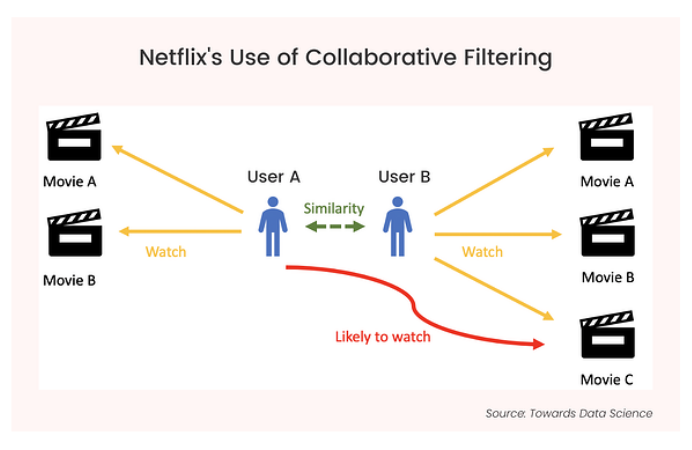
\includegraphics[width=0.8\textwidth]{pic1.png}
    \caption{Basic Flow of a Recommender System}
    \label{fig:pic1}
\end{figure}

\section{Why Focus on Collaborative Methods and Matrix Factorization in This Project}

This project primarily focuses on collaborative filtering and matrix factorization because they have shown strong performance in scenarios where rich user-item interaction data is available. Collaborative filtering’s ability to recommend based on user similarity and its flexibility across different domains makes it a popular choice for large-scale recommender systems. 

Furthermore, matrix factorization techniques, such as Singular Value Decomposition (SVD) and CUR decomposition, allow us to handle large, sparse datasets efficiently by reducing dimensionality and uncovering latent factors driving user preferences. These methods are especially useful in improving the performance of recommender systems, particularly when dealing with sparse ratings matrices, which is a common challenge in real-world applications.

By focusing on these techniques, the project aims to demonstrate the effectiveness of collaborative filtering and matrix factorization in providing accurate and scalable recommendations in environments where user preferences and behavior are key to understanding item relevance.

% Insert images here
\begin{figure}[htbp]
    \centering
    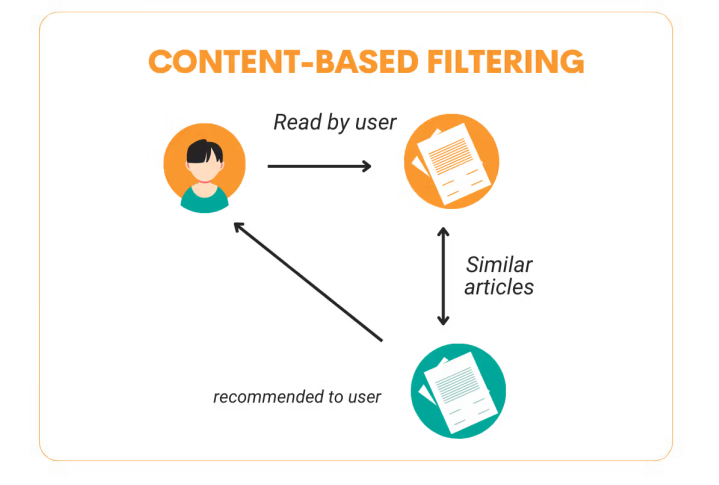
\includegraphics[width=0.8\textwidth]{pic2.png}
    \caption{Design Overview of the Matrix Factorization Model}
    \label{fig:pic2}
\end{figure}

% Insert images here
\begin{figure}[htbp]
    \centering
    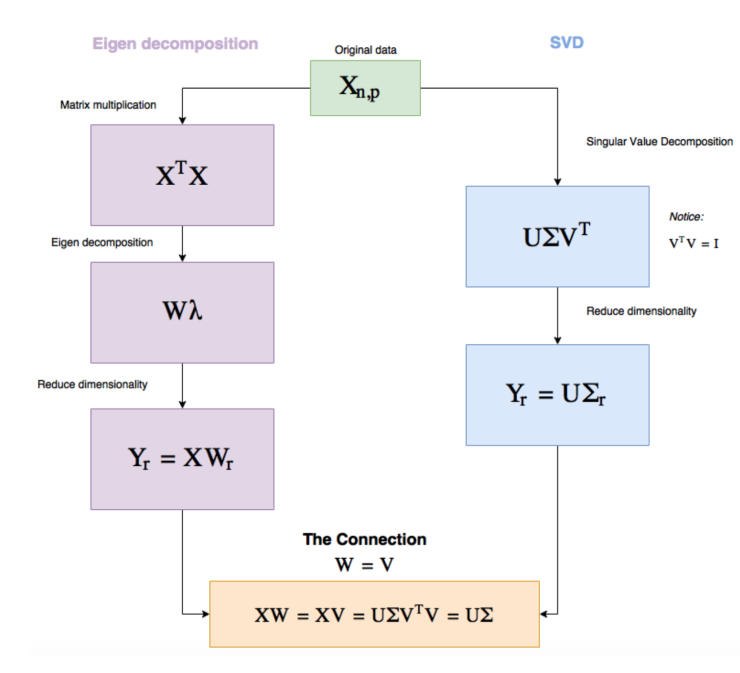
\includegraphics[width=0.8\textwidth]{pic3.png}
    \caption{Flow of the Collaborative Filtering Approach}
    \label{fig:pic3}
\end{figure}

\chapter{Dataset Details}

The Jester Online Joke Recommender Dataset (\url{https://goldberg.berkeley.edu/jester-data/}) is a widely used dataset in recommender system research, offering insights into how users rate jokes. It contains 4.1 million ratings from 73,421 users who rated 100 jokes, with ratings ranging from -10.00 to +10.00. The dataset was collected between April 1999 and May 2003 and is freely available for research purposes with proper acknowledgment.

\section{Dataset Structure}

The dataset is structured as a user-item matrix, where:
\begin{itemize}
    \item Rows represent users, and columns represent jokes.
    \item Each entry in the matrix corresponds to a user’s rating for a particular joke.
    \item Missing or null ratings are marked as "99."
\end{itemize}

Key statistics of the dataset:
\begin{itemize}
    \item The matrix has dimensions of 73,421 × 100 (users × jokes).
    \item Ratings range from -10.00 to +10.00, reflecting the user's enjoyment or dislike of a joke.
\end{itemize}

\section{Significance of Dense Submatrices}

Within this large matrix, certain submatrices are "dense," meaning that most users have rated those items. For instance:
\begin{itemize}
    \item The submatrix formed by columns \{5, 7, 8, 13, 15, 16, 17, 18, 19, 20\} is dense, as nearly all users have rated those jokes.
\end{itemize}

This density indicates that some jokes are universally popular, making it easier to identify patterns of preferences and similarities among users.

\section{Justification for Dataset Suitability}

The Jester dataset is highly suitable for collaborative filtering-based recommender systems due to the following reasons:
\begin{itemize}
    \item \textbf{Large, Sparse, and Real-world Matrix:} Collaborative filtering algorithms thrive on this type of data, as user preferences can be compared to generate recommendations.
    \item \textbf{Continuous Ratings:} Unlike integer-based ratings, the continuous scale (-10.00 to +10.00) provides finer granularity, allowing for more nuanced predictions.
    \item \textbf{Matrix Factorization:} The sparsity of the matrix allows researchers to explore techniques like matrix factorization to handle missing data, a common challenge in real-world recommender systems.
    \item \textbf{Long History and Large User Base:} The dataset's long collection period and large, anonymized user base make it ideal for testing collaborative filtering algorithms, especially for addressing challenges like the cold start problem (new users/items with no historical data) and data sparsity.
\end{itemize}

\section{Summary}

In summary, the Jester dataset is particularly well-suited for testing collaborative filtering and matrix factorization techniques due to its:
\begin{itemize}
    \item Size and sparsity.
    \item Continuous nature of ratings.
    \item Real-world applicability.
\end{itemize}

It serves as an excellent resource for experimenting with recommender system challenges and gaining a deeper understanding of user preferences in a real-world context.


\chapter{Methodology Overview}

This chapter outlines the methodology used to implement and evaluate recommender system algorithms, focusing on Singular Value Decomposition (SVD) and CUR decomposition.

\section{Data Cleaning and Preparation}

\begin{itemize}
    \item The dataset is read from an Excel file and transformed into a utility matrix.
    \item This matrix serves as the basis for matrix factorization techniques like SVD and CUR.
\end{itemize}

\section{Implementation of Algorithms}

\subsection{Singular Value Decomposition (SVD)}
\begin{itemize}
    \item SVD decomposes a matrix into three components: \( U \), \( \Sigma \), and \( V \).
    \item This technique reduces the matrix’s dimensionality, making it suitable for recommendation tasks by approximating the original matrix.
\end{itemize}

\subsection{CUR Decomposition}
\begin{itemize}
    \item CUR selects a subset of rows and columns to approximate the original matrix.
    \item This method is computationally efficient, especially for large datasets.
\end{itemize}

\section{Step-by-Step Code Breakdown}

\subsection{SVD Class}

\begin{enumerate}
    \item \textbf{Reading the Data:}
    \begin{itemize}
        \item The \texttt{dataframe()} method reads the utility matrix from the Excel file.
    \end{itemize}
    \item \textbf{Matrix Calculations:}
    \begin{itemize}
        \item The \texttt{Ucalc()} and \texttt{Vcalc()} methods calculate the \( U \) and \( V \) matrices by multiplying the utility matrix and its transpose, then finding eigenvalues and eigenvectors.
        \item The \texttt{Sigma()} method computes the \( \Sigma \) matrix by taking square roots of the eigenvalues.
    \end{itemize}
    \item \textbf{Dimensionality Reduction:}
    \begin{itemize}
        \item The \texttt{DimentionReduction()} method retains only the most significant singular values, which capture the majority of the data's energy.
    \end{itemize}
    \item \textbf{Error Estimation:}
    \begin{itemize}
        \item \textbf{RMSE:} Root Mean Squared Error evaluates the approximation accuracy.
        \item \textbf{TopK:} Error estimation for the top \( K \) values.
        \item \textbf{Spearman’s Correlation:} Measures rank correlation between predicted and actual data.
    \end{itemize}
\end{enumerate}

\subsection{CUR Class}

\begin{enumerate}
    \item \textbf{Reading the Data:}
    \begin{itemize}
        \item The \texttt{dataframe()} method loads the utility matrix from the Excel file.
    \end{itemize}
    \item \textbf{Probability Distribution:}
    \begin{itemize}
        \item The \texttt{probdistribution()} method computes the probabilities for selecting rows and columns.
    \end{itemize}
    \item \textbf{Matrix Construction:}
    \begin{itemize}
        \item \texttt{C\_calc()} and \texttt{R\_calc()} methods construct the \( C \) and \( R \) matrices by randomly selecting columns and rows based on probabilities.
        \item The \texttt{U\_calc()} method computes the \( U \) matrix using the \( C \) and \( R \) matrices and SVD-like approximations.
    \end{itemize}
    \item \textbf{Error Estimation:}
    \begin{itemize}
        \item Similar to SVD, the \texttt{ErrorEstimate()} method calculates RMSE, TopK error, and Spearman’s correlation.
    \end{itemize}
\end{enumerate}

\section{Code Flow}

\subsection{SVD Flow}
\begin{enumerate}
    \item \textbf{Read Data:} Load the matrix from an Excel file.
    \item \textbf{Calculate \( U \) and \( V \):} Perform matrix decomposition into \( U \), \( \Sigma \), and \( V \).
    \item \textbf{Error Estimation:} Compute RMSE, TopK, and Spearman’s correlation for evaluation.
\end{enumerate}

\subsection{CUR Flow}
\begin{enumerate}
    \item \textbf{Read Data:} Load the matrix from an Excel file.
    \item \textbf{Probability Distribution:} Calculate probabilities for selecting rows and columns.
    \item \textbf{Matrix Construction:} Create \( C \), \( R \), and \( U \) matrices.
    \item \textbf{Error Estimation:} Evaluate the approximation using RMSE, TopK, and Spearman’s correlation.
\end{enumerate}

\section{Usage}

\subsection{SVD}
\begin{itemize}
    \item Load the utility matrix from an Excel file.
    \item Decompose the matrix into \( U \), \( \Sigma \), and \( V \) using SVD.
    \item Optionally, reduce dimensionality by retaining significant singular values.
    \item Estimate errors using RMSE, TopK, and Spearman’s correlation.
\end{itemize}

\subsection{CUR}
\begin{itemize}
    \item Load the utility matrix from the Excel file.
    \item Compute the probability distribution for selecting rows and columns.
    \item Construct \( C \), \( R \), and \( U \) matrices.
    \item Estimate errors in approximation using RMSE, TopK, and Spearman’s correlation.
\end{itemize}

\chapter{Results and Analysis}

This chapter compares the performance of two matrix factorization methods, Singular Value Decomposition (SVD) and CUR (Column-Row), based on accuracy and computational efficiency. The analysis evaluates their suitability for tasks like recommendation systems.

\section{Performance Metrics}

\subsection{Accuracy Comparison}
The accuracy of the approximation is evaluated using the following metrics:

\begin{itemize}
    \item \textbf{Root Mean Squared Error (RMSE):} Measures the deviation between predicted and actual values. Lower RMSE values indicate better approximation accuracy.
    \item \textbf{TopK Error:} Evaluates the error for the top \( K \) predicted values, critical for recommendation systems. Smaller errors indicate better performance.
    \item \textbf{Spearman's Rank Correlation:} Quantifies the rank correlation between predicted and actual values. Higher values indicate better prediction quality.
\end{itemize}

\subsection{Computational Efficiency}
The computational efficiency of the algorithms is assessed based on:
\begin{itemize}
    \item \textbf{Time Taken:} The time required to factorize the matrix and compute approximations.
    \item \textbf{Memory Usage:} The memory consumed during execution, including storage for input data and intermediate calculations.
\end{itemize}

\section{Observations on Accuracy and Computational Efficiency}

\subsection{Accuracy}
\begin{enumerate}[a.]
    \item \textbf{SVD:} 
    \begin{itemize}
        \item Consistently achieves lower RMSE and TopK errors compared to CUR.
        \item Demonstrates higher Spearman's rank correlation, indicating superior approximation quality.
        \item This makes SVD particularly suitable for applications requiring high accuracy, such as recommendation systems.
    \end{itemize}
    \item \textbf{CUR:}
    \begin{itemize}
        \item While less accurate than SVD, CUR provides reasonably good approximations for large-scale datasets.
        \item Its slightly higher RMSE and TopK errors, along with lower rank correlation, suggest trade-offs in accuracy.
    \end{itemize}
\end{enumerate}

\subsection{Computational Efficiency}
\begin{enumerate}[a.]
    \item \textbf{CUR:}
    \begin{itemize}
        \item Processes the matrix faster than SVD, making it more efficient in terms of runtime.
        \item Consumes less memory due to its focus on a subset of rows and columns, which reduces computational complexity.
        \item These characteristics make CUR a viable choice for real-time applications or environments with resource constraints.
    \end{itemize}
    \item \textbf{SVD:}
    \begin{itemize}
        \item Requires more processing time due to the decomposition of the entire matrix.
        \item Consumes significantly more memory, especially for large matrices.
        \item While computationally intensive, its accuracy justifies its use in applications where precision is crucial.
    \end{itemize}
\end{enumerate}


\chapter*{References}

\begin{enumerate}
    \item Koren, Y., Bell, R., \& Volinsky, C. (2009). Matrix factorization techniques for recommender systems. \textit{Computer}, \textit{42}(8), 30-37. \\
    DOI: \url{https://doi.org/10.1109/MC.2009.263}

    \item Drineas, P., \& Mahoney, M. W. (2005). On the Approximability of Low-Rank Matrix Approximation Problems. \textit{Proceedings of the 16th Annual ACM-SIAM Symposium on Discrete Algorithms (SODA '05)}, 1-10. \\
    DOI: \url{https://doi.org/10.1137/1.9781611973751.1}

    \item Candes, E. J., \& Recht, B. (2009). Exact Matrix Completion via Convex Optimization. \textit{Foundations of Computational Mathematics}, \textit{9}(6), 717-772. \\
    DOI: \url{https://doi.org/10.1007/s10208-009-9045-5}
\end{enumerate}

\end{document}